\section{Makahiki}
The feature set of WattDepot creates attractive infrastructure for management of energy data, but research suggests that effective participation of consumers in a next generation smart grid requires more than simple feedback to consumers about their consumption, particularly given the passive nature of their involvement for the past 100 years.

The second component of our open source software stack, Makahiki, represents research intended to create synergy between the need to create knowledge and engagement regarding energy and the ability of so-called ``serious game'' techniques and/or energy feedback to create participation and engagement \cite{Deterding2011mt,darby-review-2006,Faruqui09,petersen-dorm-energy-reduction}. In Makahiki, online game mechanics are employed with the goal of affecting real-world energy behaviors.  The ultimate goal is to not just affect energy behaviors during the course of the game, but to produce long lasting, sustained change in energy behaviors and outlooks by participants. Figure \ref{fig:makahiki-architecture} illustrates the architecture of Makahiki.

\begin{figure}
\begin{center}
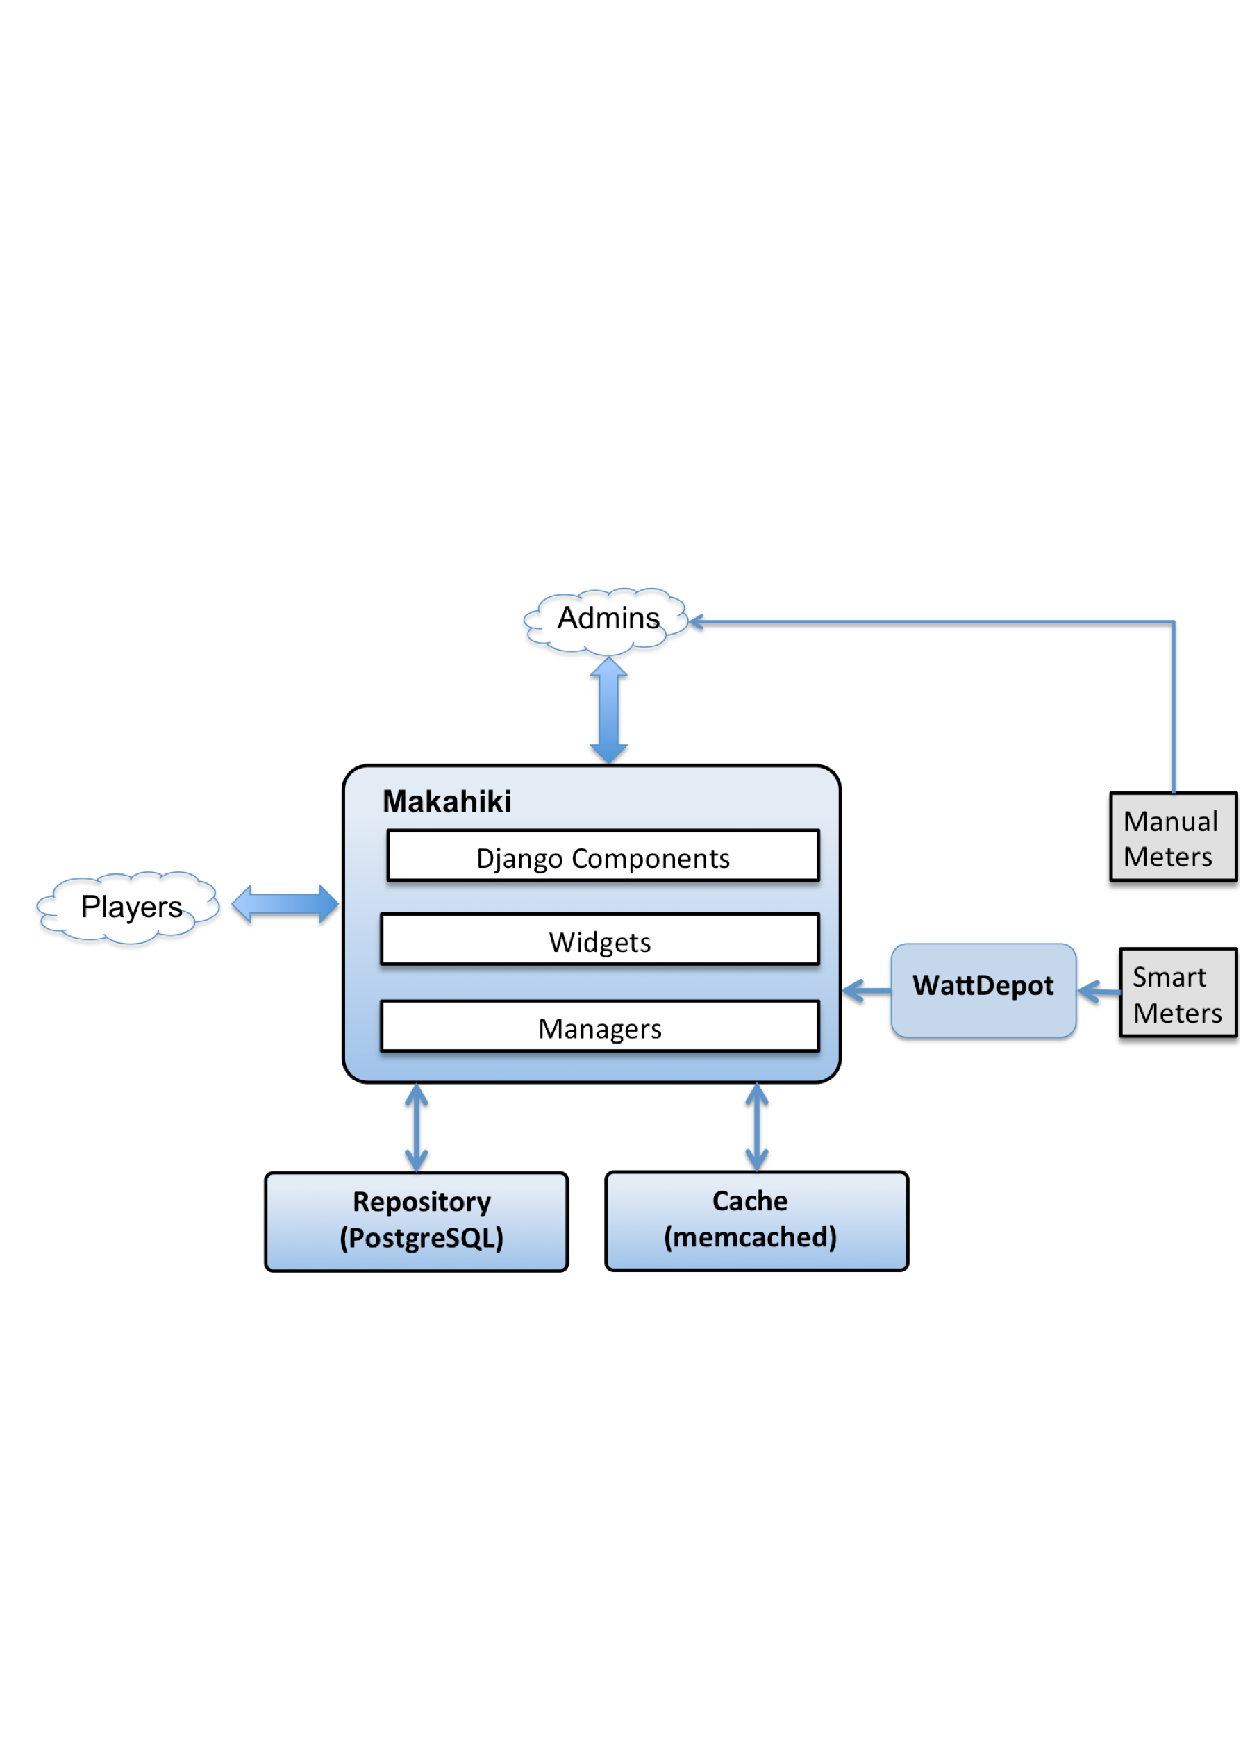
\epsfig{file=makahiki-system-architecture, width=3in}
\end{center}
\caption{Architecture of Makahiki}
\label{fig:makahiki-architecture}
\end{figure}

Makahiki consists of a configurable game engine that can be customized to the needs of different organizations.  It includes a library of pre-built game ``widgets'' that implement a variety of game mechanics.  Using the widgets, an organization can create a custom energy challenge in which players can compete individually and/or in teams to earn the most points by reducing their energy consumption as well as by learning about energy concepts in general.  Some of the pre-built widgets include:

The {\em Smart Grid Game widget} is the primary place players go to learn about energy issues and earn points.  The Smart Grid Game supports four different kinds of actions: activities, commitments, events, and excursions.

The {\em Daily Energy Goal Game widget} provides a way for players to earn points by reducing their current consumption from a baseline that is typically determined prior to the challenge. Both the historical baseline data and the current consumption is typically provided by API calls from Makahiki to an underlying WattDepot server.

The {\em Raffle Game widget} provides a way to incentivize participation from all individuals, even those who are not in the running for a top prize. For every 25 points a player earns, they receive one virtual raffle ticket. Players can dynamically allocate their tickets to any raffle prizes they are interested in at any time, up to the end of the raffle.

The {\em Social and Referral Bonus widgets} provide game mechanics that help encourage participation by providing additional points to players who participate in activities with other players and/or facilitate the entry of new players into an energy challenge.
